\section{Dataset clusters comparison}

		\begin{figure*}[ht!]
			\centering
			\subfloat[Zernike coefficients]{%
				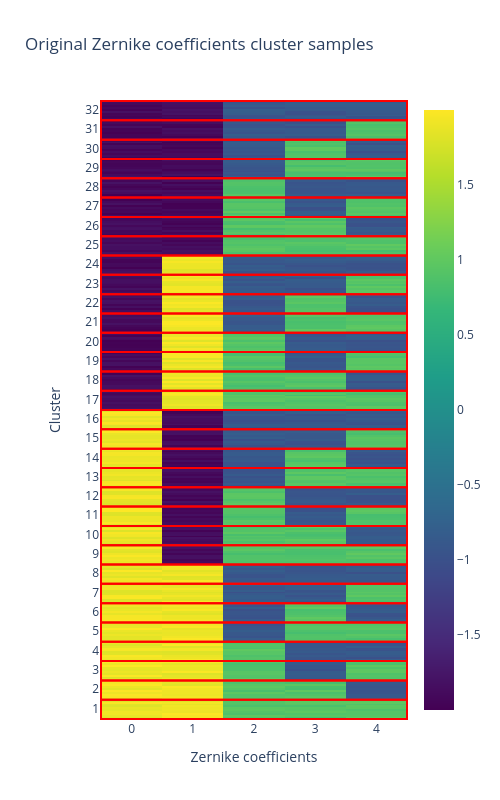
\includegraphics[width=0.22\textwidth]{mdid-5mzernikecoefficientsoriginalgridclusters.png}}
			\hspace{\fill}
			\subfloat[LP coefficients]{%
				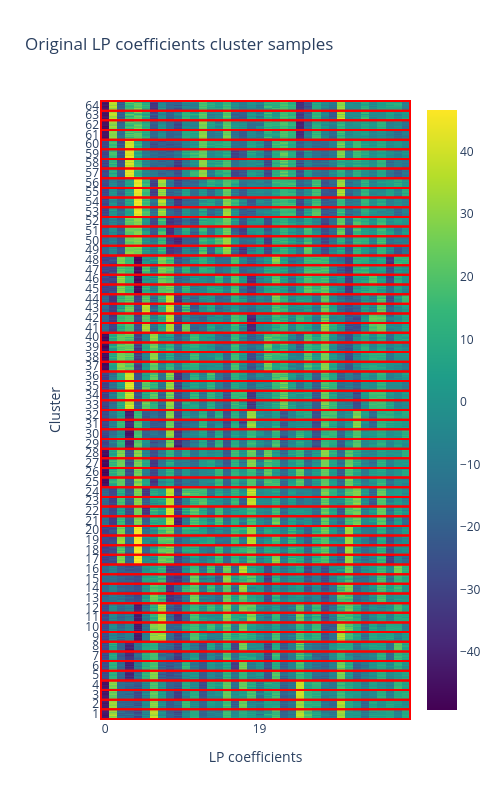
\includegraphics[width=0.22\textwidth]{mdid-9mlpcoefficientsoriginalgridclusters.png}}
			\hspace{\fill}
			\subfloat[Output fluxes]{%
				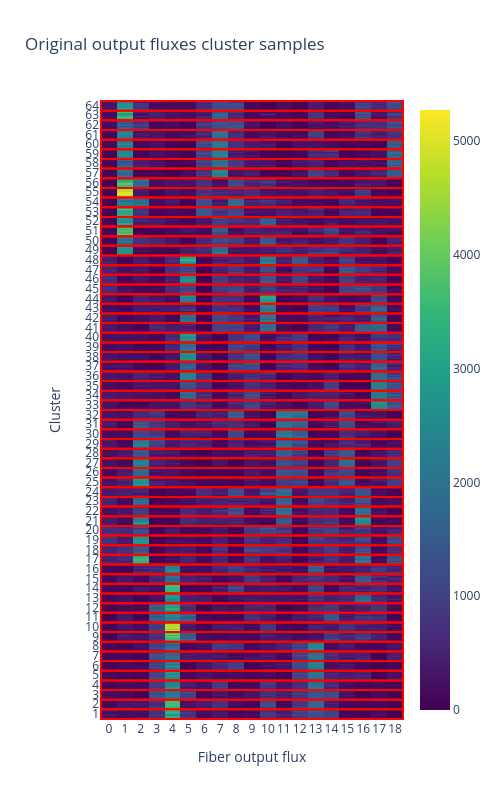
\includegraphics[width=0.22\textwidth]{mdid-9moutputfluxesoriginalgridclusters.png}}
			\hspace{\fill}
			\subfloat[PCA PSF Intensities]{%
				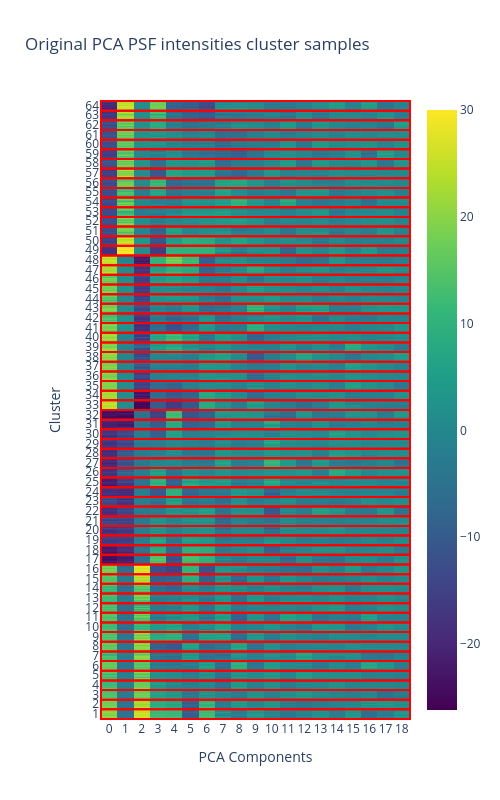
\includegraphics[width=0.22\textwidth]{mdid-9mpcaintensitiesoriginalgridclusters.png}}
			\hspace{\fill}
			\caption{Original clusters from the datasets}
		\end{figure*}
		\FloatBarrier
		
		\begin{figure*}[ht!]
			\centering
			\subfloat[Zernike coefficients]{%
				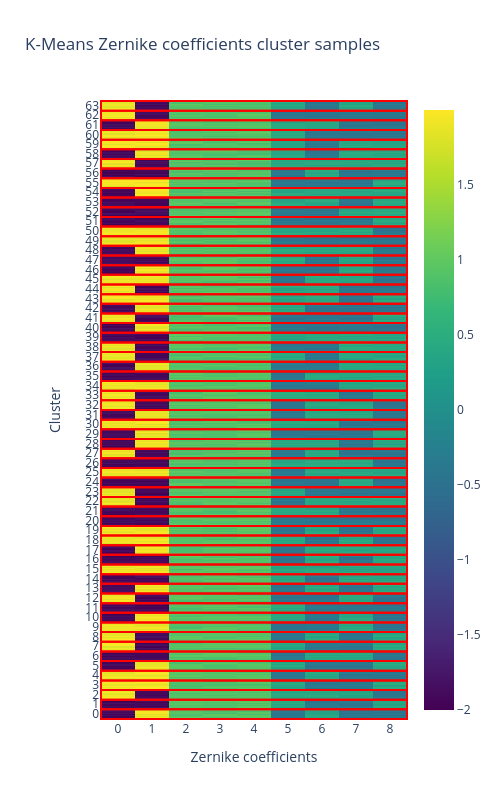
\includegraphics[width=0.22\textwidth]{mdid-9mzernikecoefficientsK-Meansgridclusters.png}}
			\hspace{\fill}
			\subfloat[LP coefficients]{%
				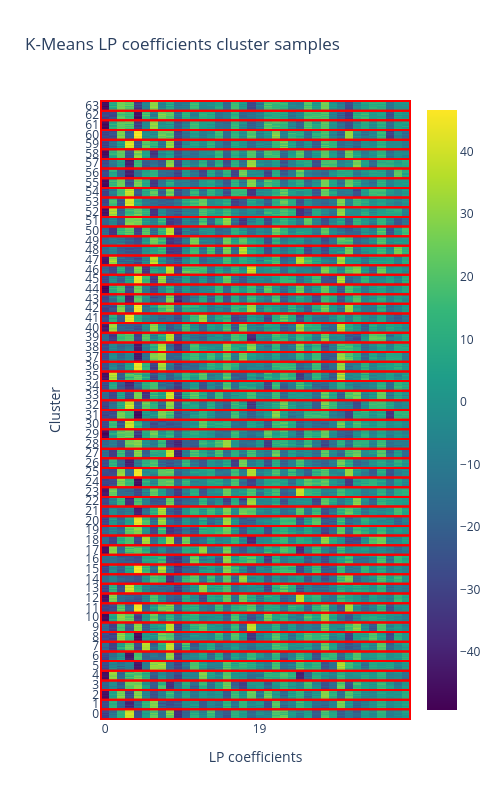
\includegraphics[width=0.22\textwidth]{mdid-9mlpcoefficientsK-Meansgridclusters.png}}
			\hspace{\fill}
			\subfloat[Output fluxes]{%
				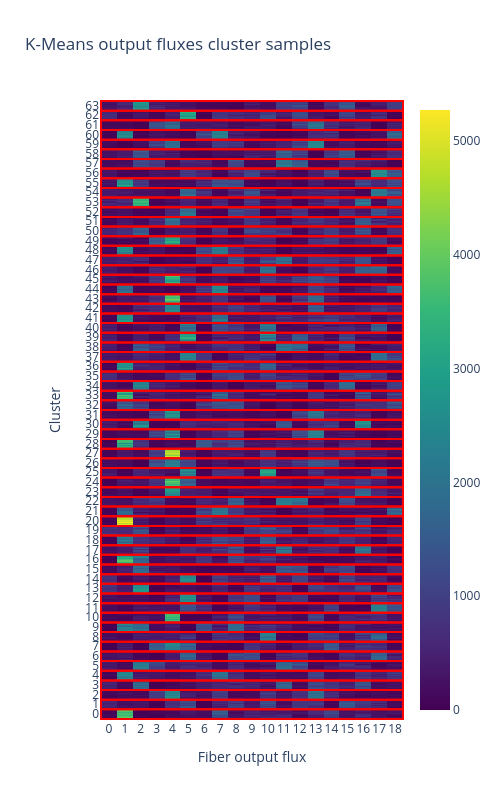
\includegraphics[width=0.22\textwidth]{mdid-9moutputfluxesK-Meansgridclusters.png}}
			\hspace{\fill}
			\subfloat[PCA PSF Intensities]{%
				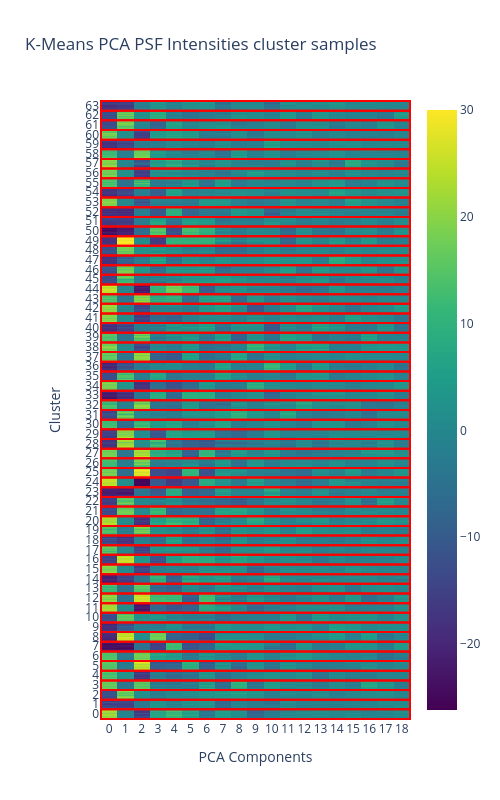
\includegraphics[width=0.22\textwidth]{mdid-9mpcaintensitiesK-Meansgridclusters.png}}
			\hspace{\fill}
			\caption{K-Means clusters from the datasets}
		\end{figure*}
		\FloatBarrier
		
		\begin{figure*}[ht!]
			\centering
			\subfloat[Zernike coefficients]{%
				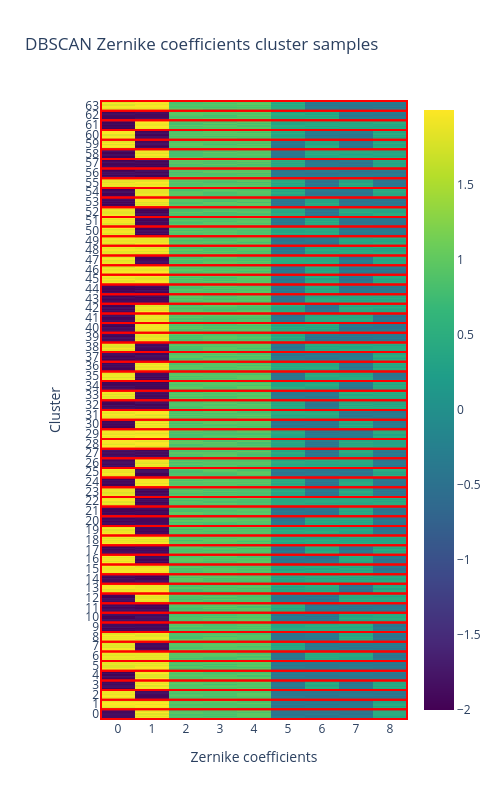
\includegraphics[width=0.22\textwidth]{mdid-9mzernikecoefficientsDBSCANgridclusters.png}}
			\hspace{\fill}
			\subfloat[LP coefficients]{%
				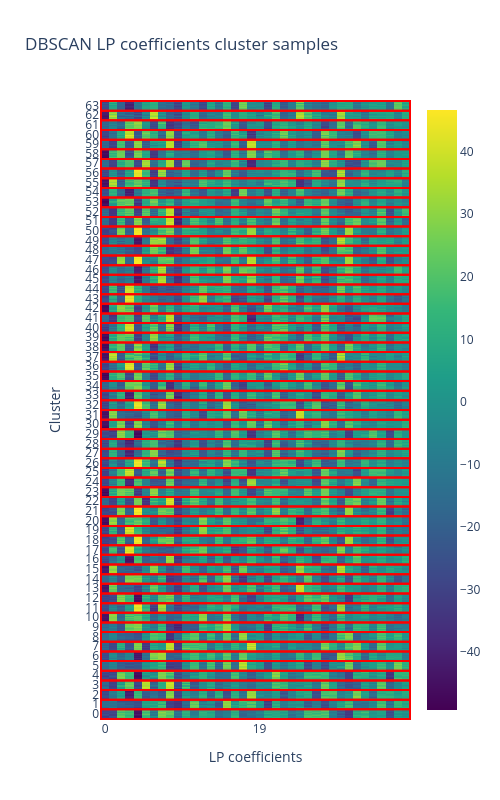
\includegraphics[width=0.22\textwidth]{mdid-9mlpcoefficientsDBSCANgridclusters.png}}
			\hspace{\fill}
			\subfloat[Output fluxes]{%
				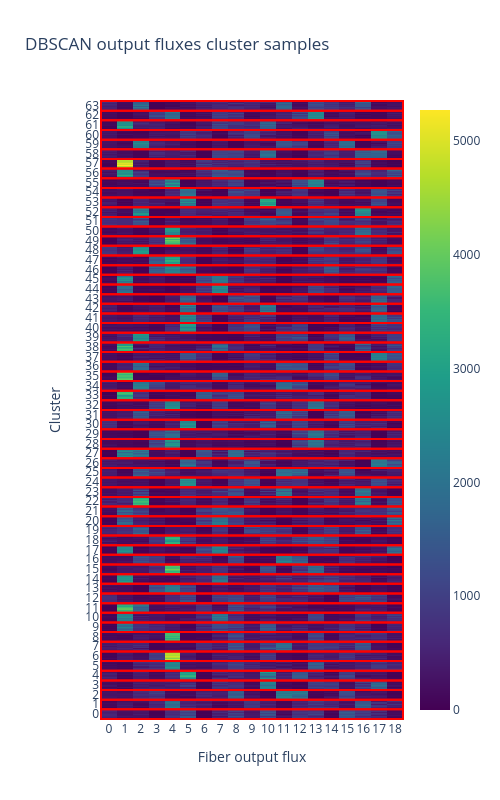
\includegraphics[width=0.22\textwidth]{mdid-9moutputfluxesDBSCANgridclusters.png}}
			\hspace{\fill}
			\subfloat[PCA PSF Intensities]{%
				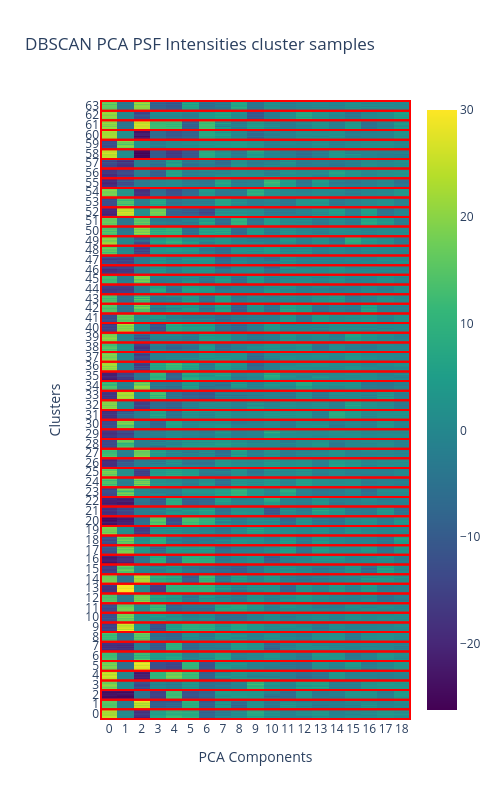
\includegraphics[width=0.22\textwidth]{mdid-9mpcaintensitiesDBSCANgridclusters.png}}
			\hspace{\fill}
			\caption{DBSCAN clusters from the datasets}
		\end{figure*}
		\FloatBarrier
		
		\begin{figure*}[ht!]
			\centering
			\subfloat[Zernike coefficients]{%
				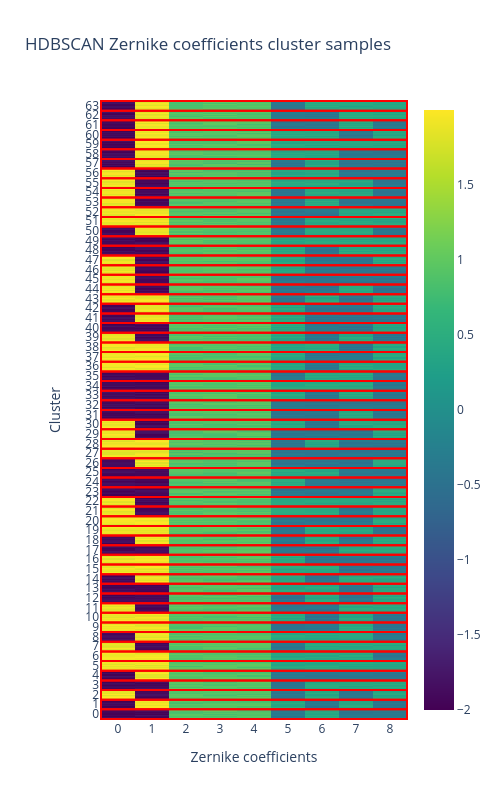
\includegraphics[width=0.22\textwidth]{mdid-9mzernikecoefficientsHDBSCANgridclusters.png}}
			\hspace{\fill}
			\subfloat[LP coefficients]{%
				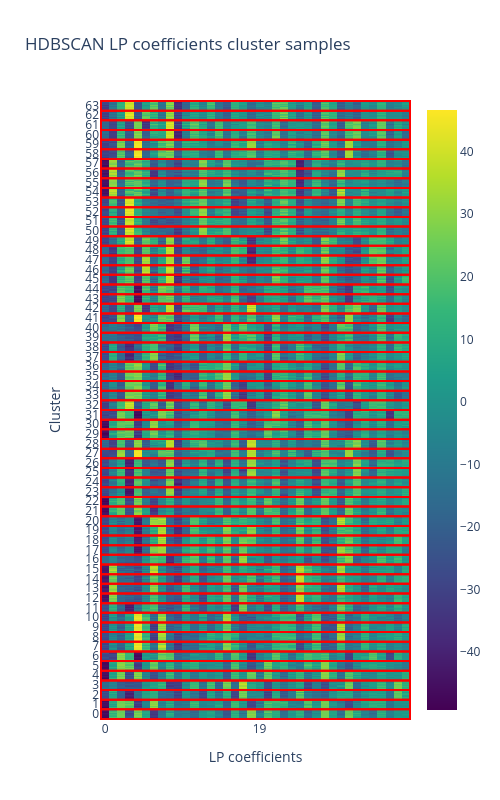
\includegraphics[width=0.22\textwidth]{mdid-9mlpcoefficientsHDBSCANgridclusters.png}}
			\hspace{\fill}
			\subfloat[Output fluxes]{%
				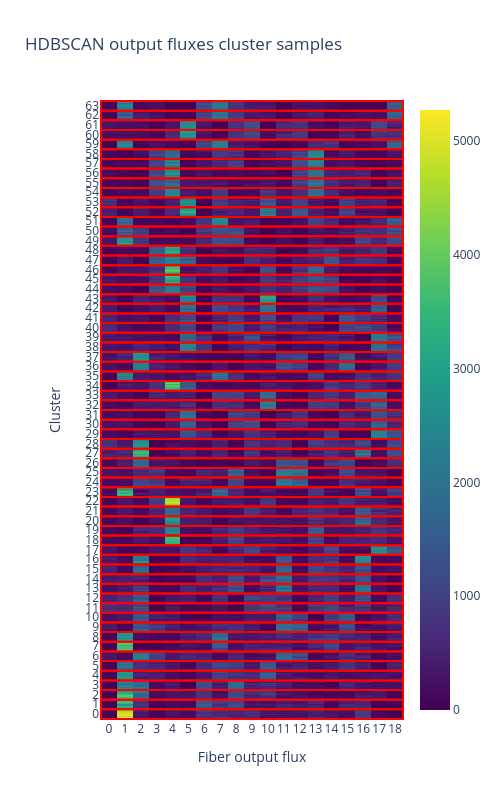
\includegraphics[width=0.22\textwidth]{mdid-9moutputfluxesHDBSCANgridclusters.png}}
			\hspace{\fill}
			\subfloat[PCA PSF Intensities]{%
				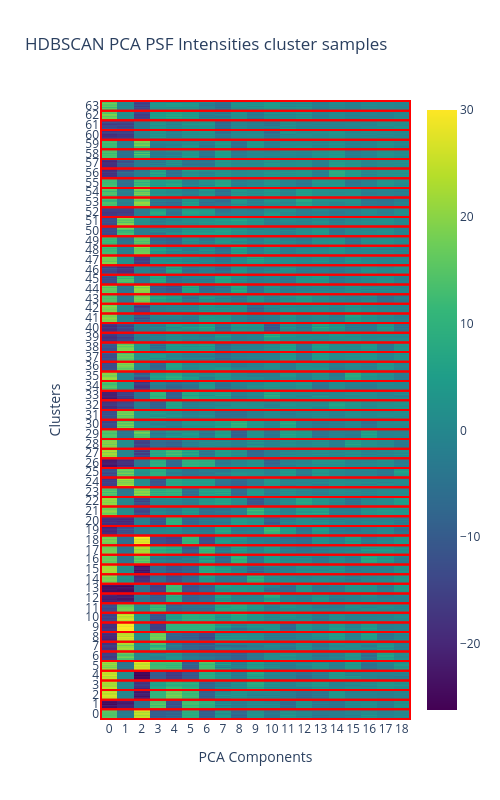
\includegraphics[width=0.22\textwidth]{mdid-9mpcaintensitiesHDBSCANgridclusters.png}}
			\hspace{\fill}
			\caption{HDBSCAN clusters from the datasets}
		\end{figure*}
		\FloatBarrier
		
		\begin{figure*}[ht!]
			\centering
			\subfloat[Zernike coefficients]{%
				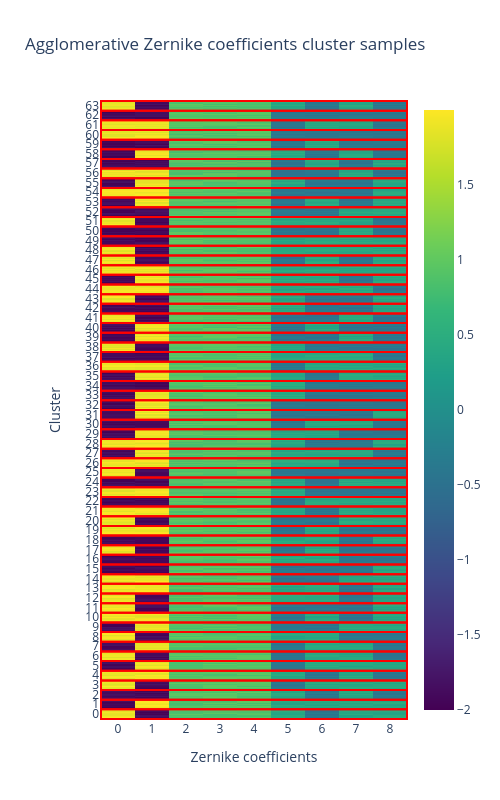
\includegraphics[width=0.22\textwidth]{mdid-9mzernikecoefficientsAgglomerativegridclusters.png}}
			\hspace{\fill}
			\subfloat[LP coefficients]{%
				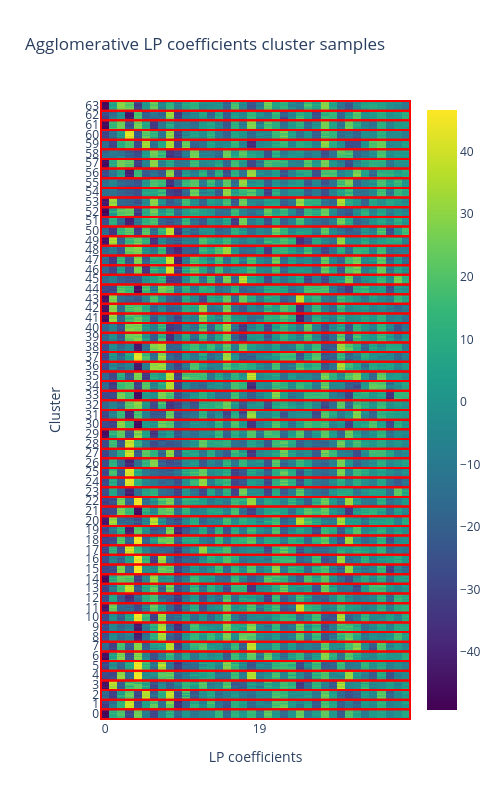
\includegraphics[width=0.22\textwidth]{mdid-9mlpcoefficientsAgglomerativegridclusters.png}}
			\hspace{\fill}
			\subfloat[Output fluxes]{%
				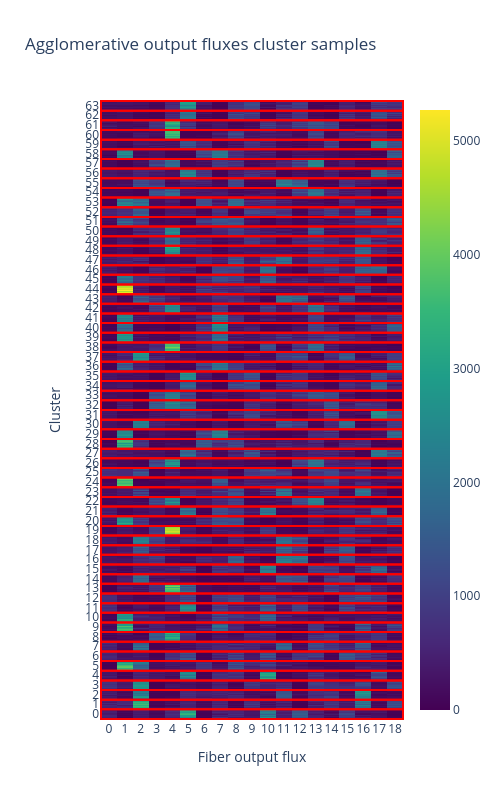
\includegraphics[width=0.22\textwidth]{mdid-9moutputfluxesAgglomerativegridclusters.png}}
			\hspace{\fill}
			\subfloat[PCA PSF Intensities]{%
				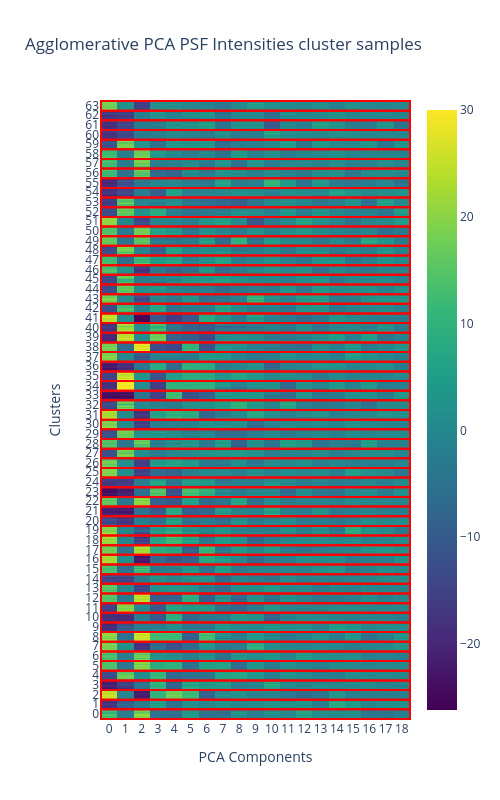
\includegraphics[width=0.22\textwidth]{mdid-9mpcaintensitiesAgglomerativegridclusters.png}}
			\hspace{\fill}
			\caption{Agglomerative clusters from the datasets}
		\end{figure*}
		\FloatBarrier